% =====================================================================
% AGILE Brief 2 — Multi-page LinkedIn Dashboard
% Author: Usman Almuarif Mashood
% Compile with:  xelatex AGILE_Brief2_Dashboard.tex
% =====================================================================

\documentclass[11pt,landscape,letterpaper]{article}

\usepackage[letterpaper,landscape,
            top=1.2cm,bottom=1.4cm,left=1.6cm,right=1.6cm]{geometry}
\usepackage{fontspec}
\usepackage{xcolor}
\usepackage{tikz}
\usepackage[most]{tcolorbox}
\usepackage{tabularx}
\usepackage{array}
\usepackage{enumitem}
\usepackage{anyfontsize}
\usepackage{fancyhdr}
\usepackage{setspace}
\usepackage{graphicx}

% --- Fonts (XeLaTeX): use system sans if Inter not available -------------
\IfFontExistsTF{Inter}{%
  \setmainfont{Inter}
  \setsansfont{Inter}
}{%
  \IfFontExistsTF{DejaVu Sans}{%
    \setmainfont{DejaVu Sans}
    \setsansfont{DejaVu Sans}
  }{%
    \setmainfont{Latin Modern Sans}
    \setsansfont{Latin Modern Sans}
  }%
}
\renewcommand{\familydefault}{\sfdefault}

% --- Palette -------------------------------------------------------------
\definecolor{navy}{HTML}{1A3A5C}
\definecolor{gold}{HTML}{C89B3C}
\definecolor{teal}{HTML}{3B7D7D}
\definecolor{lightgrey}{HTML}{F2F2F2}
\definecolor{midgrey}{HTML}{777777}
\definecolor{paneledge}{HTML}{E4E4E4}

% --- Default text color & line spacing -----------------------------------
\color{navy}
\setlength{\parindent}{0pt}

% --- Footer --------------------------------------------------------------
\pagestyle{fancy}
\fancyhf{}
\renewcommand{\headrulewidth}{0pt}
\renewcommand{\footrulewidth}{0pt}
\fancyfoot[C]{\color{midgrey}\fontsize{8.5}{10}\selectfont
  AGILE Independent M\&E Review \,$\cdot$\, Usman Almuarif Mashood
  \,$\cdot$\, June 2026 \,$\cdot$\, github.com/Almuarif17/social-protection-me-nigeria}

% --- tcolorbox styles ----------------------------------------------------
\tcbset{
  modernpanel/.style={
    enhanced, sharp corners=northwest,
    colback=lightgrey, colframe=lightgrey,
    arc=3mm, boxsep=2mm,
    left=5mm, right=5mm, top=4mm, bottom=4mm,
    fontupper=\color{navy},
    boxrule=0pt
  },
  statbox/.style={
    enhanced,
    colback=lightgrey, colframe=lightgrey,
    arc=3mm, boxsep=2mm,
    left=3mm, right=3mm, top=4mm, bottom=4mm,
    halign=center, valign=center,
    fontupper=\color{navy}, boxrule=0pt,
    height=4.4cm
  },
  componentbox/.style={
    enhanced, sharp corners=northwest,
    colback=white, colframe=navy,
    arc=2mm, boxrule=0.8pt,
    left=4mm, right=4mm, top=3mm, bottom=3mm,
    fontupper=\color{navy},
    fonttitle=\color{white}\bfseries,
    coltitle=white, colbacktitle=navy,
    title=\strut
  },
  findingpanel/.style={
    enhanced,
    colback=lightgrey, colframe=lightgrey,
    arc=3mm, boxsep=2mm,
    left=5mm, right=5mm, top=5mm, bottom=5mm,
    fontupper=\color{navy}, boxrule=0pt
  }
}

% --- helpers -------------------------------------------------------------
% Horizontal "bar" for inline mini-charts (width is fraction of \linewidth)
\newcommand{\inlinebar}[2]{%
  % #1 = fraction (0..1), #2 = color name
  \tikz[baseline=-0.6ex]{\fill[#2] (0,0) rectangle (#1\linewidth, 0.32cm);}%
}

\begin{document}

% =====================================================================
% PAGE 1 — Cover and Hook
% =====================================================================
\thispagestyle{fancy}

\vspace*{0.4cm}

{\color{navy}\fontsize{46}{54}\selectfont\bfseries
Nigeria's Largest Bet\\[-0.05em] on Girls' Education}

\vspace{0.5cm}

{\color{gold}\fontsize{20}{26}\selectfont\bfseries
AGILE: \$1.2 Billion, 8.6 Million Girls, 18 States ---\\[-0.05em]
and the Four Things Its Measurement Framework Misses.}

\vspace{0.9cm}

\begin{minipage}{0.82\textwidth}
  \color{navy}\fontsize{12.5}{19}\selectfont
  There was a time when education in Nigeria was universally promised.
  Programmes like the Universal Primary Education scheme of 1976 underwrote
  a generation's literacy and set an ambitious standard for the nation.
  Today, the Adolescent Girls Initiative for Learning and Empowerment
  (AGILE)~--- launched in 2020~--- represents the largest gender-focused
  attempt in West African history to restore that promise of access.
  Targeting the country's poorest states, it seeks to bring millions of
  adolescent girls back into the classroom. It is an extraordinary
  investment, but as this review reveals, its success depends on
  measuring what truly matters.
\end{minipage}

\vfill

\begin{minipage}{0.6\textwidth}
  \color{midgrey}\fontsize{10}{14}\selectfont
  \textbf{\color{navy}Independent M\&E Review \,$\cdot$\, Brief 2 \,$\cdot$\, June 2026}\\
  Usman Almuarif Mashood\\
  github.com/Almuarif17/social-protection-me-nigeria
\end{minipage}

\newpage
% =====================================================================
% PAGE 2 — The Programme Timeline
% =====================================================================
\thispagestyle{fancy}

\vspace*{0.1cm}
{\color{navy}\fontsize{26}{32}\selectfont\bfseries The Programme Timeline}

\vspace{1.7cm}

\begin{center}
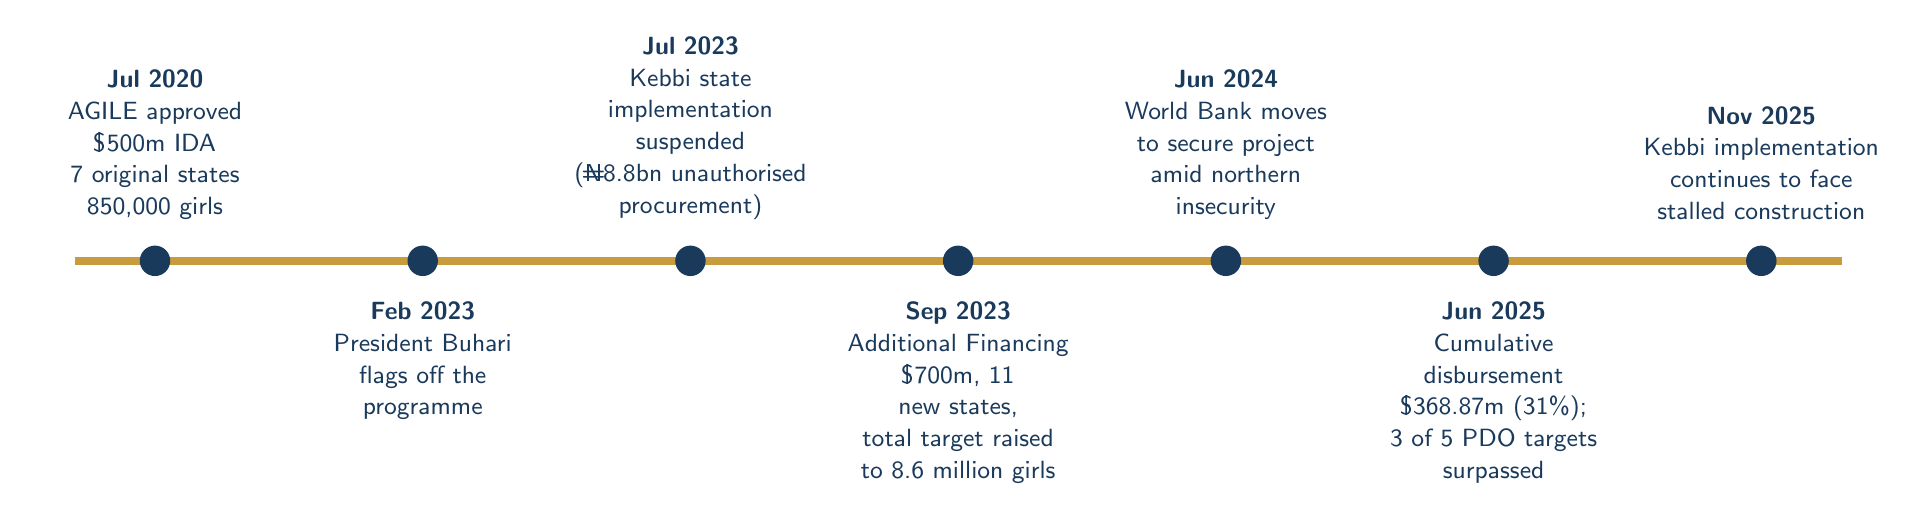
\begin{tikzpicture}[x=3.4cm, y=1cm]
  % Main line
  \draw[line width=3pt, gold] (-0.3,0) -- (6.3,0);
  % Nodes
  \foreach \x in {0,1,2,3,4,5,6} {
    \fill[navy] (\x,0) circle (5.5pt);
  }
  % Top nodes (even indices)
  \node[anchor=south, align=center, text width=3.0cm, color=navy,
        font=\fontsize{9}{11.5}\selectfont] at (0, 0.4)
        {\textbf{Jul 2020}\\AGILE approved\\\$500m IDA\\7 original states\\850,000 girls};
  \node[anchor=south, align=center, text width=3.0cm, color=navy,
        font=\fontsize{9}{11.5}\selectfont] at (2, 0.4)
        {\textbf{Jul 2023}\\Kebbi state\\implementation suspended\\(\textnaira8.8bn unauthorised\\procurement)};
  \node[anchor=south, align=center, text width=3.0cm, color=navy,
        font=\fontsize{9}{11.5}\selectfont] at (4, 0.4)
        {\textbf{Jun 2024}\\World Bank moves\\to secure project\\amid northern\\insecurity};
  \node[anchor=south, align=center, text width=3.0cm, color=navy,
        font=\fontsize{9}{11.5}\selectfont] at (6, 0.4)
        {\textbf{Nov 2025}\\Kebbi implementation\\continues to face\\stalled construction};

  % Bottom nodes (odd indices)
  \node[anchor=north, align=center, text width=3.0cm, color=navy,
        font=\fontsize{9}{11.5}\selectfont] at (1, -0.4)
        {\textbf{Feb 2023}\\President Buhari\\flags off the\\programme};
  \node[anchor=north, align=center, text width=3.0cm, color=navy,
        font=\fontsize{9}{11.5}\selectfont] at (3, -0.4)
        {\textbf{Sep 2023}\\Additional Financing\\\$700m, 11 new states,\\total target raised\\to 8.6 million girls};
  \node[anchor=north, align=center, text width=3.0cm, color=navy,
        font=\fontsize{9}{11.5}\selectfont] at (5, -0.4)
        {\textbf{Jun 2025}\\Cumulative disbursement\\\$368.87m (31\%);\\3 of 5 PDO targets\\surpassed};
\end{tikzpicture}
\end{center}

\vfill

\begin{center}
\begin{minipage}{0.85\textwidth}
  \color{navy}\fontsize{10.5}{15}\selectfont\itshape
  Source: World Bank Project Appraisal Document (P170664, 2020), Additional Financing
  documents (P179281, 2023), Implementation Status \& Results Reports through June 2025;
  Guardian Nigeria (2023, 2024); Punch Newspapers (2025).
\end{minipage}
\end{center}

\newpage
% =====================================================================
% PAGE 3 — What AGILE Is + What It Has Achieved
% =====================================================================
\thispagestyle{fancy}

\vspace*{0.1cm}

\begin{minipage}[t]{0.46\textwidth}
  {\color{navy}\fontsize{22}{28}\selectfont\bfseries What AGILE Is}

  \vspace{0.6cm}

  \begin{tcolorbox}[componentbox, title={\bfseries\fontsize{11}{14}\selectfont Component 1\,---\, Safe \& Accessible Learning Spaces}]
    \fontsize{10}{13}\selectfont
    Addresses the supply side of secondary education. Provides School Improvement
    Grants for new classrooms, sanitation facilities, water infrastructure,
    and rehabilitation of existing buildings.
  \end{tcolorbox}

  \vspace{0.35cm}

  \begin{tcolorbox}[componentbox, title={\bfseries\fontsize{11}{14}\selectfont Component 2\,---\, Fostering an Enabling Environment}]
    \fontsize{10}{13}\selectfont
    Addresses demand and social norms. Includes the \textit{Madubi} communication
    campaign, advocacy with traditional and religious leaders, life-skills
    and digital-literacy training, and financial incentives for the poorest
    households.
  \end{tcolorbox}

  \vspace{0.35cm}

  \begin{tcolorbox}[componentbox, title={\bfseries\fontsize{11}{14}\selectfont Component 3\,---\, System Strengthening}]
    \fontsize{10}{13}\selectfont
    Provides institutional infrastructure: technical assistance, M\&E,
    Grievance Redress Mechanisms, environmental and social safeguards,
    and federal--state capacity building.
  \end{tcolorbox}
\end{minipage}
\hfill
\begin{minipage}[t]{0.50\textwidth}
  {\color{navy}\fontsize{22}{28}\selectfont\bfseries What AGILE Has Achieved}

  \vspace{0.6cm}

  \begin{itemize}[label={\color{gold}\textbullet}, itemsep=0.55cm, leftmargin=*, topsep=0pt]
    \item {\color{navy}\fontsize{22}{26}\selectfont\bfseries 5{,}000+}\\
          \fontsize{11}{15}\selectfont
          classrooms constructed or rehabilitated by April 2023
    \item {\color{navy}\fontsize{22}{26}\selectfont\bfseries 8{,}400+}\\
          \fontsize{11}{15}\selectfont toilet units installed
    \item {\color{navy}\fontsize{22}{26}\selectfont\bfseries 48\% $\rightarrow$ 67\%}\\
          \fontsize{11}{15}\selectfont
          Kano JSS gross enrolment ratio (2021 $\rightarrow$ 2025)
    \item {\color{navy}\fontsize{22}{26}\selectfont\bfseries 38\% $\rightarrow$ 59\%}\\
          \fontsize{11}{15}\selectfont
          Kano SSS gross enrolment ratio over the same period
    \item {\color{navy}\fontsize{22}{26}\selectfont\bfseries 3 of 5}\\
          \fontsize{11}{15}\selectfont
          Year-5 PDO targets surpassed (World Bank IRM, June 2025)
  \end{itemize}
\end{minipage}

\newpage
% =====================================================================
% PAGE 4 — Methodology
% =====================================================================
\thispagestyle{fancy}

\vspace*{0.7cm}
\begin{center}
\begin{minipage}{0.88\textwidth}
  \color{navy}\fontsize{16}{23}\selectfont\bfseries
  This brief is built on the World Bank's anonymised AGILE-IE Baseline
  Survey 2023 --- the same dataset the programme's official impact evaluation
  will use.
\end{minipage}
\end{center}

\vspace{1.3cm}

\noindent
\begin{tabularx}{\textwidth}{@{}XXXX@{}}
  \begin{tcolorbox}[statbox]
    {\color{gold}\fontsize{34}{40}\selectfont\bfseries 8{,}223}\\[0.2cm]
    \fontsize{11}{15}\selectfont\bfseries adolescent girls\\surveyed
  \end{tcolorbox} &
  \begin{tcolorbox}[statbox]
    {\color{gold}\fontsize{34}{40}\selectfont\bfseries 8{,}007}\\[0.2cm]
    \fontsize{11}{15}\selectfont\bfseries caregivers\\interviewed
  \end{tcolorbox} &
  \begin{tcolorbox}[statbox]
    {\color{gold}\fontsize{34}{40}\selectfont\bfseries 270}\\[0.2cm]
    \fontsize{11}{15}\selectfont\bfseries school principals\\surveyed
  \end{tcolorbox} &
  \begin{tcolorbox}[statbox]
    {\color{gold}\fontsize{34}{40}\selectfont\bfseries 3}\\[0.2cm]
    \fontsize{11}{15}\selectfont\bfseries of the 7 original\\AGILE states
  \end{tcolorbox}
\end{tabularx}

\vspace{1.2cm}

\begin{center}
\begin{minipage}{0.88\textwidth}
  \fontsize{11}{16}\selectfont\color{navy}
  \textbf{Analytical approach.} Cross-sectional descriptive analysis in Python
  (pandas, NumPy, Matplotlib). Reproducibility guaranteed via the published
  Google Colab notebook in the public repository.\\[0.45cm]
  \textbf{Limitations.} The data captures baseline pre-programme conditions
  only, preventing causal impact attribution. The survey scope covers three
  northern states (Kaduna, Kano, Katsina) out of the expanded 18-state
  footprint. All measures are self-reported via CAPI interview.
\end{minipage}
\end{center}

\newpage
% =====================================================================
% PAGE 5 — Findings (Part 1): Digital + Aspirations
% =====================================================================
\thispagestyle{fancy}

\vspace*{0.05cm}
{\color{navy}\fontsize{20}{26}\selectfont\bfseries The Four Findings\, (I)}

\vspace{0.45cm}

% ---- Panel 1 ----
\begin{tcolorbox}[findingpanel]
  \begin{minipage}[c]{0.55\textwidth}
    {\color{gold}\fontsize{36}{42}\selectfont\bfseries 1 in 6}\\[0.25cm]
    \fontsize{11.5}{16.5}\selectfont\bfseries
    Only 17\% of SS1 girls in AGILE-area schools have ever used a mobile
    phone independently. Fewer than 1\% have ever touched a computer.\\[0.35cm]
    {\color{teal}\itshape\bfseries M\&E gap:}~{\color{teal}\itshape
    The Results Framework counts trainees but does not record their
    pre-training digital exposure.}
  \end{minipage}\hfill
  \begin{minipage}[c]{0.40\textwidth}
    \fontsize{10}{14}\selectfont\bfseries
    Adolescent girls with prior device exposure\\[0.35cm]
    \fontsize{10}{12}\selectfont Mobile phone (any)\\
    \inlinebar{0.51}{navy}~\textbf{17\%}\\[0.18cm]
    \fontsize{10}{12}\selectfont Smartphone\\
    \inlinebar{0.18}{navy}~\textbf{6\%}\\[0.18cm]
    \fontsize{10}{12}\selectfont Computer\\
    \inlinebar{0.02}{navy}~\textbf{<1\%}
  \end{minipage}
\end{tcolorbox}

\vspace{0.35cm}

% ---- Panel 2 ----
\begin{tcolorbox}[findingpanel]
  \begin{minipage}[c]{0.55\textwidth}
    {\color{gold}\fontsize{36}{42}\selectfont\bfseries 73\% $\rightarrow$ 32\%}\\[0.25cm]
    \fontsize{11.5}{16.5}\selectfont\bfseries
    Share of caregivers aspiring to a bachelor's degree or higher for
    their daughter, Kaduna vs Katsina. Aspirations fall by more than half
    moving north.\\[0.35cm]
    {\color{teal}\itshape\bfseries M\&E gap:}~{\color{teal}\itshape
    No aspiration baseline against which Component 2's social-norm
    change can be measured.}
  \end{minipage}\hfill
  \begin{minipage}[c]{0.40\textwidth}
    \fontsize{10}{14}\selectfont\bfseries
    Caregivers aspiring to bachelor's or higher\\[0.35cm]
    \fontsize{10}{12}\selectfont Kaduna\\
    \inlinebar{0.73}{navy}~\textbf{73\%}\\[0.18cm]
    \fontsize{10}{12}\selectfont Kano\\
    \inlinebar{0.43}{navy}~\textbf{43\%}\\[0.18cm]
    \fontsize{10}{12}\selectfont Katsina\\
    \inlinebar{0.32}{navy}~\textbf{32\%}
  \end{minipage}
\end{tcolorbox}

\newpage
% =====================================================================
% PAGE 6 — Findings (Part 2): Food security + Seating
% =====================================================================
\thispagestyle{fancy}

\vspace*{0.05cm}
{\color{navy}\fontsize{20}{26}\selectfont\bfseries The Four Findings\, (II)}

\vspace{0.45cm}

% ---- Panel 3 ----
\begin{tcolorbox}[findingpanel]
  \begin{minipage}[c]{0.55\textwidth}
    {\color{gold}\fontsize{36}{42}\selectfont\bfseries 1 in 5}\\[0.25cm]
    \fontsize{11.5}{16.5}\selectfont\bfseries
    Households in the AGILE-IE sample that skipped meals in the past
    seven days. Rises to 1 in 4 (27\%) in Katsina.\\[0.35cm]
    {\color{teal}\itshape\bfseries M\&E gap:}~{\color{teal}\itshape
    No food-security targeting indicator to verify the
    financial-incentive sub-component reach.}
  \end{minipage}\hfill
  \begin{minipage}[c]{0.40\textwidth}
    \fontsize{10}{14}\selectfont\bfseries
    Households that skipped meals in the last 7 days\\[0.35cm]
    \fontsize{10}{12}\selectfont Katsina\\
    \inlinebar{0.81}{navy}~\textbf{27\%}\\[0.18cm]
    \fontsize{10}{12}\selectfont Kaduna\\
    \inlinebar{0.66}{navy}~\textbf{22\%}\\[0.18cm]
    \fontsize{10}{12}\selectfont Kano\\
    \inlinebar{0.39}{navy}~\textbf{13\%}
  \end{minipage}
\end{tcolorbox}

\vspace{0.35cm}

% ---- Panel 4 ----
\begin{tcolorbox}[findingpanel]
  \begin{minipage}[c]{0.55\textwidth}
    {\color{gold}\fontsize{36}{42}\selectfont\bfseries 26\%}\\[0.25cm]
    \fontsize{11.5}{16.5}\selectfont\bfseries
    Share of surveyed AGILE-area SS1 schools that have enough classroom
    seats for the girls already enrolled. Three in four do not.\\[0.35cm]
    {\color{teal}\itshape\bfseries M\&E gap:}~{\color{teal}\itshape
    Infrastructure indicators count classrooms built, not seats provided.}
  \end{minipage}\hfill
  \begin{minipage}[c]{0.40\textwidth}
    \fontsize{10}{14}\selectfont\bfseries
    School infrastructure reality check\\[0.35cm]
    \fontsize{10}{12}\selectfont Any toilet available\\
    \inlinebar{0.95}{navy}~\textbf{95\%}\\[0.18cm]
    \fontsize{10}{12}\selectfont Drinking water available\\
    \inlinebar{0.92}{navy}~\textbf{92\%}\\[0.18cm]
    \fontsize{10}{12}\selectfont Sufficient classroom seats\\
    \inlinebar{0.26}{gold}~\textbf{26\%}
  \end{minipage}
\end{tcolorbox}

\newpage
% =====================================================================
% PAGE 7 — The Critical Gap and Five Recommendations
% =====================================================================
\thispagestyle{fancy}

\vspace*{0.2cm}
{\color{navy}\fontsize{26}{32}\selectfont\bfseries The Critical Gap}

\vspace{0.5cm}

\begin{minipage}{0.96\textwidth}
  \color{navy}\fontsize{13}{19}\selectfont
  AGILE's Results Framework measures \textit{what the programme does}~---
  girls trained, classrooms built, incentives paid~--- with adequate
  precision. It does not adequately measure the conditions that determine
  whether those outputs convert into outcomes: whether trainees had prior
  exposure to benefit from training, whether caregivers' aspirations are
  rising, whether the households most in need of support are receiving it,
  and whether girls actually have a seat in which to learn.
\end{minipage}

\vspace{1.1cm}
{\color{navy}\fontsize{17}{22}\selectfont\bfseries
Five Indicators AGILE Should Add Before Midline}

\vspace{0.5cm}

\begin{enumerate}[label={\color{gold}\bfseries\fontsize{14}{16}\selectfont\arabic*.},
                 itemsep=0.4cm, leftmargin=*, topsep=0pt]
  \item \fontsize{11.5}{16}\selectfont\bfseries
        Pre-training digital-exposure intake form.\hspace{0.25em}
        {\color{teal}\itshape\mdseries
        Addresses the inability to distinguish digital learning gains
        from prior-exposure advantage.}
  \item \fontsize{11.5}{16}\selectfont\bfseries
        Caregiver educational aspiration measure.\hspace{0.25em}
        {\color{teal}\itshape\mdseries
        Addresses the lack of a baseline against which to evaluate
        Component~2's social-norm change.}
  \item \fontsize{11.5}{16}\selectfont\bfseries
        Food-security targeting verification measure.\hspace{0.25em}
        {\color{teal}\itshape\mdseries
        Addresses the lack of proof that financial incentives reach
        the most food-insecure households.}
  \item \fontsize{11.5}{16}\selectfont\bfseries
        Classroom seating-adequacy annual verification.\hspace{0.25em}
        {\color{teal}\itshape\mdseries
        Addresses the binding constraint that newly built classrooms
        often lack adequate furniture.}
  \item \fontsize{11.5}{16}\selectfont\bfseries
        Gender-disaggregated intra-household resource indicator.\hspace{0.25em}
        {\color{teal}\itshape\mdseries
        Addresses the need to track whether cash transfers specifically
        protect girls from meal shortfalls.}
\end{enumerate}

\vfill
\begin{center}
  {\color{navy}\fontsize{12}{16}\selectfont\bfseries
  Read the full 30-page brief on GitHub: \\[0.15cm]
  github.com/Almuarif17/social-protection-me-nigeria}
\end{center}

\end{document}
